\documentclass{article}

\usepackage[margin=0.5in]{geometry}
\usepackage{multicol}
\usepackage{siunitx}
\usepackage{tikz}
\usepackage{amsthm}

\theoremstyle{definition}
\newtheorem*{solution}{Solution}
\title{Solid Geometry Set B}
\author{}
\date{}

\begin{document}
\maketitle
\begin{multicols}{2}
    \begin{enumerate}
        \item What is the total surface area of a right square pyramid with a height of $12$ feet and a base with side length of $10$ feet?
            \begin{solution}
                The 12-foot altitude of this right square pyramid meets the square base at is center, which is $5$ feet away from the midpoint of a side of the square base.
                This forms a $5$-$12$-$13$ triangle, which is a Pythagorean Triple. The $13$-foot side is the slant height of each of the four triangle faces of the pyramid.
                The combined area of the four triangular faces is $4 \cdot \frac{1}{2} \cdot 10 \cdot 13 = \SI{260}{ft\squared}$.
                The area of the $10$-foot by $10$-foot square base is $10 \cdot 10 = \SI{100}{ft\squared}$.
                The total surface area of the pyramid, then, is $260 + 100 = \SI{360}{ft\squared}$.
            \end{solution}
        \item This figure shows the net of a three-dimensional shape called a truncated octahedron.
            How many vertices does a truncated octahedron have?
            \begin{center}
                \includegraphics[scale=0.4]{octahedron.png}
            \end{center}
            \begin{solution}
                The figure shows $8$ hexagons, which have $8 \cdot 6 = 48$ vertices, and $6$ squares, which have $6 \cdot 4 = 24$ vertices.
                That's a total of $48 + 24 = 72$ vertices on the two-dimensional net.
                When the net is folded into a three-dimensional octahedron, two hexagons and one square meet at each vertex.
                Thus, the number of vertices on the solid is $\frac{72}{3} = 24$ vertices.
                Alternatively, since each vertex of the solid is a vertex of exactly one square, it is sufficient to count just the vertices of the $64$ squares.
                Doing so yields a total of $4 \cdot 6 = 24$ vertices for the solid.
            \end{solution}
        \item A sphere is inscribed in a cube.
            What is the ratio of the volume of the cube to that of the sphere?
            Express your answer as a common fraction in terms of $\pi$.
            \begin{solution}
                The diameter of the sphere is equal to the side length $s$ of the cube.
                The volume of the cube $s^3$, and the volume of the sphere is $\frac{s^3}{\frac{\pi s^3}{6}} = \frac{6}{\pi}$.
                Note that because the sphere is inside the cube, the ratio has to be greater than $1$, of course.
                It is interesting that the ratio is almost $2$ (because $\pi \approx 3.1$), meaning the sphere takes up only a little more than half the space inside the cube.
            \end{solution}
        \item In the figure shown, a triangular pyramid has been cut off the corner of the cube so that an equilateral triangle face is formed.
            If each corner of the cube is cut off in this manner, what is the maximum sum of the number of faces, edges, and vertices on the new polyhedron?
            \begin{center}
                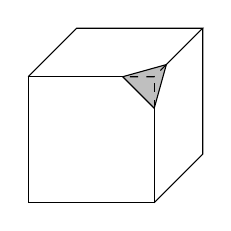
\begin{tikzpicture}[scale=0.4]
                    \draw (3,4,4) -- (0,4,4) -- (0,0,4) -- (4,0,4) -- (4,3,4);
                    \draw (0,4,4) -- (0,4,0) -- (4,4,0) -- (4,4,3);
                    \draw (4,4,0) -- (4,0,0) -- (4,0,4);
                    \draw[fill=lightgray] (4,4,3) -- (3,4,4) -- (4,3,4) -- cycle;
                    \draw[dashed] (4,4,3) -- (4,4,4) -- (3,4,4);
                    \draw[dashed] (4,3,4) -- (4,4,4);
                \end{tikzpicture}
            \end{center}
            \begin{solution}
                A cube has $6$ faces, $12$ edges, and $8$ vertices. When each vertex is cut off, $1$ new equilateral triangle face is created, though the size of the triangle can vary.
                There is a net gain of at most, $3$ edges for a maximum of $8 \cdot 3 = 24$ additional edges.
                There is also a net gain of at most, $2$ vertices, for a maximum of $8 \cdot 2 = 16$ additional vertices.
                At most, the sum of the number of faces, edges, and vertices will be $(6 + 8) + (12 + 24) + (8 + 16) = 14 + 36 +24 = 74$.
                Note that this maximum can be achieved if the cube is cut so that for each new triangle face none of its vertices reaches the midpoint of an edge of the cube (Fig. 1).
                Otherwise, the resulting solid would have fewer edges and vertices (Fig. 2).
                \begin{center}
                    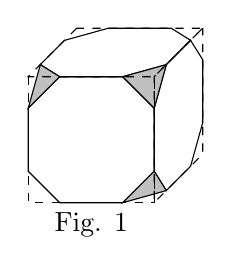
\begin{tikzpicture}[scale=0.4]
                        \draw (3,4,4) -- (1,4,4) -- (0,3,4) -- (0,1,4) -- (1,0,4) -- (3,0,4) -- (4,1,4) -- (4,3,4) -- cycle;
                        \draw (1,4,4) -- (0,4,3) -- (0,4,1) -- (1,4,0) -- (3,4,0) -- (4,4,1) -- (4,4,3) -- (3,4,4) -- cycle;
                        \draw (4,4,1) -- (4,3,0) -- (4,1,0) -- (4,0,1) -- (4,0,3) -- (4,1,4) -- (4,3,4) -- (4,4,3) -- cycle;
                        \draw[fill=lightgray] (3,4,4) -- (4,4,3) -- (4,3,4) -- cycle;
                        \draw[fill=lightgray] (0,3,4) -- (1,4,4) -- (0,4,3) -- cycle;
                        \draw[fill=lightgray] (3,0,4) -- (4,0,3) -- (4,1,4) -- cycle;
                        \draw[dashed] (0,4,0) -- (0,4,4) -- (4,4,4) -- (4,4,0) -- cycle;
                        \draw[dashed] (0,4,4) -- (0,0,4) -- (4,0,4) node[midway, below] {Fig. 1} -- (4,4,4) -- cycle;
                        \draw[dashed] (4,4,0) -- (4,4,4) -- (4,0,4) -- (4,0,0) -- cycle;
                    \end{tikzpicture}
                    \hspace{1cm}
                    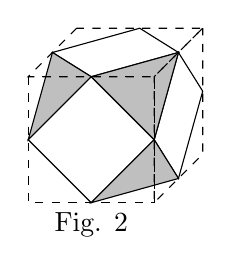
\begin{tikzpicture}[scale=0.4]
                        \draw (2,4,4) -- (2,4,4) -- (0,2,4) -- (0,2,4) -- (2,0,4) -- (2,0,4) -- (4,2,4) -- (4,2,4) -- cycle;
                        \draw (2,4,4) -- (0,4,2) -- (0,4,2) -- (2,4,0) -- (2,4,0) -- (4,4,2) -- (4,4,2) -- (2,4,4) -- cycle;
                        \draw (4,4,2) -- (4,2,0) -- (4,2,0) -- (4,0,2) -- (4,0,2) -- (4,2,4) -- (4,2,4) -- (4,4,2) -- cycle;
                        \draw[fill=lightgray] (2,4,4) -- (4,4,2) -- (4,2,4) -- cycle;
                        \draw[fill=lightgray] (0,2,4) -- (2,4,4) -- (0,4,2) -- cycle;
                        \draw[fill=lightgray] (2,0,4) -- (4,0,2) -- (4,2,4) -- cycle;
                        \draw[dashed] (0,4,0) -- (0,4,4) -- (4,4,4) -- (4,4,0) -- cycle;
                        \draw[dashed] (0,4,4) -- (0,0,4) -- (4,0,4) node[midway, below] {Fig. 2}  -- (4,4,4) -- cycle;
                        \draw[dashed] (4,4,0) -- (4,4,4) -- (4,0,4) -- (4,0,0) -- cycle;
                    \end{tikzpicture}
                \end{center}
            \end{solution}
        \item When a cone's height is decrease by a factor of four, to maintain the same volume, the radius must be increased by a factor of two, or $100\%$.
            When the cone's height is decreased by a factor of three, by what percent must the radius be increased to maintain the same volume?
            Express your answer to the nearest whole number.
            \begin{solution}
                The volume of a cone is $\frac{1}{3} \cdot \pi \cdot r^2 \cdot h$.
                Notice that we multiply by the height $h$ and the square of the radius $r$.
                This is why doubling the radius can compensate for reducing the height by one-fourth.
                We get the same volume because $2^2 \cdot \frac{1}{4} = \frac{4}{4} = 1$.
                If we decrease the height to $\frac{1}{3}$ of what is was, the radius has to increase by a number that when squared is $3$.
                That number is $\sqrt{3}$.
                Since $\sqrt{3} \approx 1.73$, the radius must increase by a factor of $1.73 - 1 \approx 0.73$, or $73\%$.
            \end{solution}
    \end{enumerate}
\end{multicols}
\end{document}